\section{Analyse structurelle}
\begin{obj}
Cette partie a pour objectif d'analyser la structure du train d'atterrissage et de déterminer la variation d'inclinaison du vérin amortisseur.
\end{obj}



\begin{marginfigure}
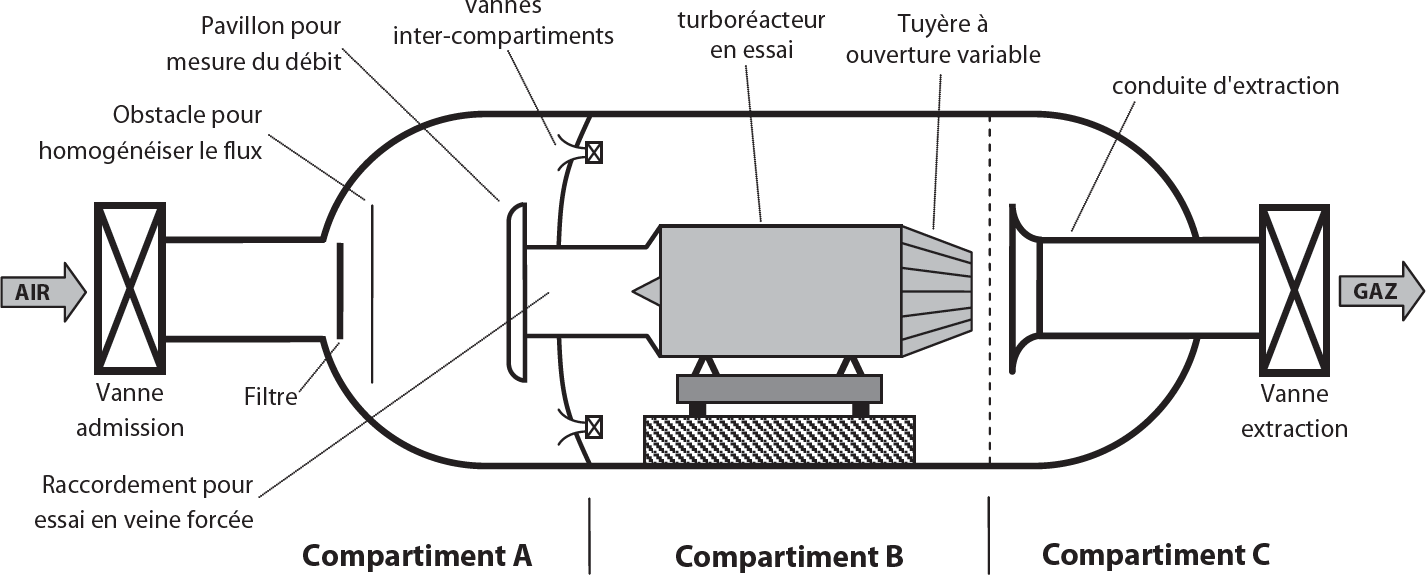
\includegraphics[width=\linewidth]{fig_02.png}
\caption{Strucutre de la jambe du train principal \label{fig_sia2014_02}}
\end{marginfigure}

On considère que l'hélicoptère est en phase d'approche. Le train n'est donc pas en contact avec le sol. Le solide 1 est solidaire du châssis de l'hélicoptère. 

\question{Déterminer le degré d'hyperstisme du modèle. Le cas échéant proposer un modèle isostatique.}




On donne le schéma cinématique de la structure du train principal (figure \ref{fig_sia2014_03}).
\begin{figure}[H]
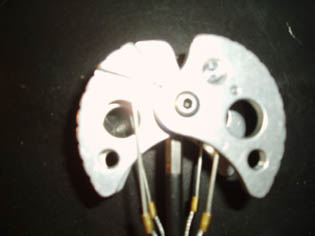
\includegraphics[width=\linewidth]{fig_03.png}
\caption{Schéma cinématique plan de la strucutre du train principal \label{fig_sia2014_03}}
\end{figure}

\question{Déterminer la variation $\Delta \beta$ de l'angle $\beta$ quand $\alpha$ varie de 0 à 45\degres. Conclure.} 

